\documentclass[journal,12pt,twocolumn]{IEEEtran}
\usepackage{cite}
\usepackage{amsmath,amssymb,amsfonts,amsthm}
\usepackage{algorithmic}
\usepackage{graphicx}
\usepackage{textcomp}
\usepackage{xcolor}
\usepackage{txfonts}
\usepackage{listings}
\usepackage{enumitem}
\usepackage{mathtools}
\usepackage{gensymb}
\usepackage{comment}
\usepackage[breaklinks=true]{hyperref}
\usepackage{tkz-euclide} 
\usepackage{circuitikz}
\usepackage{pgfplots}                            
\usepackage[latin1]{inputenc}                                
\usepackage{color}                                            
\usepackage{array}                                            
\usepackage{longtable}                                       
\usepackage{calc}                                             
\usepackage{multirow}                                         
\usepackage{hhline}                                           
\usepackage{ifthen}                                           
\usepackage{lscape}

\newtheorem{theorem}{Theorem}[section]
\newtheorem{problem}{Problem}
\newtheorem{proposition}{Proposition}[section]
\newtheorem{lemma}{Lemma}[section]
\newtheorem{corollary}[theorem]{Corollary}
\newtheorem{example}{Example}[section]
\newtheorem{definition}[problem]{Definition}
\newcommand{\BEQA}{\begin{eqnarray}}
\newcommand{\EEQA}{\end{eqnarray}}
\newcommand{\define}{\stackrel{\triangle}{=}}
\theoremstyle{remark}
\newtheorem{rem}{Remark}

\usepackage{pgfplots}
\pgfplotsset{width=7cm,compat=1.16}

\begin{document}

\bibliographystyle{IEEEtran}
\vspace{3cm}

\title{NCERT Physics 12.7. Q20}
\author{EE23BTECH11204- Ashley Ann Benoy$^{*}$% <-this % stops a space
}
\maketitle
\newpage
\bigskip

\bibliographystyle{IEEEtran}

\textbf{Question}

A series LCR circuit with 
\(L = 0.12 \, \text{H}\),
\(C = 480 \times 10^{-9} \, \text{F}\), 
\(R=23 \, \Omega\)
is connected to a 230 V variable frequency supply.

(a) What is the source frequency for which the current amplitude is maximum? Obtain this maximum value.

(b) What is the source frequency for which the average power absorbed by the circuit is maximum? Obtain the value of this maximum power.

(c) For which frequencies of the source is the power transferred to the circuit half the power at resonant frequency? What is the current amplitude at these frequencies?

(d) What is the Q-factor of the given circuit?

\textbf{Solution:}

Given parameters are:
\setcounter{table}{0} % Set the table number to 1
\textbf{
\begin{table}[htbp]
\centering
\caption{Given Data}
\label{tab:data}
\begin{tabular}{|c|c|c|}
\hline
\textbf{Symbol} & \textbf{Value} & \textbf{Parameter} \\
\hline
\(L\) & \(0.12 \, \text{H}\) & Inductance \\
\(C\) & \(480 \, \text{nF}\) & Capacitance \\
\(R\) & \(23 \, \Omega\) & Resistance \\
\(V\) & \(230 \, \text{V}\) & Supply voltage \\
\hline
\end{tabular}
\end{table}
}



% goes into figs

\begin{figure}[htb]
    \centering
    \begin{circuitikz} 
        \draw (0,0)
        to[sinusoidal voltage source, v=$V$] (0,2) % Voltage source
        to[R, l=$R$] (2,2) % Resistor
        to[L, l=$sL$] (4,2) % Inductor
        to[C, l=$\frac{1}{sC}$] (4,0); % Capacitor
        \draw (4,2) to[short, -o] (5,2) node[right] {Terminal}; % Terminal label
        \draw (0,0) to[short, -o] (5,0) node[right] {Terminal}; % Terminal label
    \end{circuitikz}
    \caption{Circuit diagram with sinusoidal voltage source, resistor, inductor, and capacitor.}
    \label{fig:circuit}
\end{figure}


The impedance of the above circuit is given as:
\begin{align}
  H(s) &= \dfrac{V(s)}{I(s)}\\
     H(s) &= R + sL + \dfrac{1}{sC}\\
     \implies H(j\omega) &= R + j\omega L + \dfrac{1}{j\omega C}
\end{align}
\begin{align}
\implies \lvert H(j\omega) \rvert &= \sqrt{R^2 + \left(\omega L - \dfrac{1}{\omega C}\right)^2}
\end{align}\\\\
\begin{enumerate}
    \item \textbf{Part (a):}

    At resonance, the circuit becomes purely resistive. The reactances of capacitor and inductor cancel out as follows:

    \begin{align}
        Ls + \frac{1}{sC} &= 0 \\
        \implies s &= j\frac{1}{\sqrt{LC}} = j\omega
    \end{align}

    The current (\(I\)) is given by Ohm's Law as:

    \begin{align}
        I &= \frac{V}{Z} = \frac{V}{R + j(\omega L - \frac{1}{\omega C})}
    \end{align}

    Substitute the expression for \(Z\) into the current equation:

    \begin{align}
        I &= \frac{V}{R + j(\omega L - \frac{1}{\omega C})} \\
    \end{align}

    \begin{align}
        |I| &= \frac{V}{\sqrt{(\omega L- \frac{1}{\omega C})^2 + (R)^2}}
    \end{align}

    The source frequency for maximum current amplitude is given by:

    \begin{align}
        \omega_{\text{max}} &= \frac{1}{\sqrt{LC}}
    \end{align}

    Substitute the values and calculate:

    \begin{align}
        \omega_{\text{max}} &\approx 4166.67 \, \text{rad/s}
    \end{align}

    \item \textbf{Part (b):}

    The source frequency for which the average power absorbed by the circuit is maximum is the same as the resonance frequency.

    \begin{align}
        I_{\text{max}} &= \frac{V}{Z_{\text{total}}} = \frac{V}{R}
    \end{align}

    At resonance, \(Z_{\text{total}} = R\), so \(I_{\text{max}} = \frac{V}{R}\).

    \begin{align}
        P_{\text{avg}} &= \frac{1}{2} I_{\text{max}}^2 R
    \end{align}

    Substitute \(I_{\text{max}} = \frac{V}{R}\) into the expression for \(P_{\text{avg}}\):

    \begin{align}
        P_{\text{avg}} &= \frac{1}{2} \left(\frac{V}{R}\right)^2 R
    \end{align}

    \begin{align}
        P_{\text{avg}} &= \frac{1}{2} \frac{V^2}{R} \label{eq:9}
    \end{align}

    Substitute the given values and calculate:

    \begin{align}
        P_{\text{avg}} &= 1150 \, \text{W}
    \end{align}

    \item \textbf{Part (c):}

    The power in the circuit is given by \(P_{\text{max}} = i_{\text{max}}^2 R\). At half power frequencies, \(P = \frac{P_{\text{max}}}{2}\), and the current is \(\frac{i_{\text{max}}}{\sqrt{2}}\). Then, \(V = \frac{i_{\text{max}}}{\sqrt{2}} Z\).

\begin{align}
Z^2 = R^2 + \left(2\pi f L - \frac{1}{2\pi f C}\right)^2
\end{align}
\begin{align}
2R^2=  R^2 + \left(2\pi f L - \frac{1}{2\pi f C}\right)^2
\end{align}

    \begin{align}
        R^2 &= \left(2\pi f L - \frac{1}{2\pi f C}\right)^2 \\
        R &= \pm \left(2\pi f L - \frac{1}{2\pi f C}\right)
    \end{align}

    This leads to two equations:

    \begin{align}
        R &= 2\pi f_1 L - \frac{1}{2\pi f_1 C} \\
        R &= \frac{1}{2\pi f_2 C} - 2\pi f_2 L
    \end{align}

    Solving these equations gives the half power frequencies \(f_1\) and \(f_2\).

    Additionally, the bandwidth \(\Delta\omega\) is related to \(R\) and \(L\) by \(\Delta\omega = \frac{R}{2L}\). In terms of angular frequency \(\omega\), we have \(\omega_1 - \omega_2 = \frac{R}{L}\).

    \begin{align}
        \omega' &= \omega_R \pm \Delta\omega \\
        \Delta\omega &= \frac{R}{2L}
    \end{align}

    Substitute the given values and calculate:

    \begin{align}
        \Delta\omega &= 95.83 \, \text{rad/s}
    \end{align}

    Finally,

    \begin{align}
        \omega'_1 &= \omega_{\text{max}} + \Delta\omega = 4262.3 \, \text{rad/s} \\
        \omega'_2 &= \omega_{\text{max}} - \Delta\omega = 4070.87 \, \text{rad/s}
    \end{align}

    The amplitude of current at these frequencies is the RMS value, which is \(10 \, \text{A}\).

    \item \textbf{Part (d):}

    The Q-factor (\(Q\)) of a series RLC circuit is given by the formula:

    \[Q = \frac{1}{R} \sqrt{\frac{L}{C}} \label{eq:Qfact}\]

    Substitute the given values and calculate:

    \begin{align}
        Q &\approx \frac{1}{23} \sqrt{\frac{0.12}{480 \times 10^{-9}}} \\
        Q &\approx 39.6826 
    \end{align}
\end{enumerate}

\begin{figure}[h!]
  \centering
  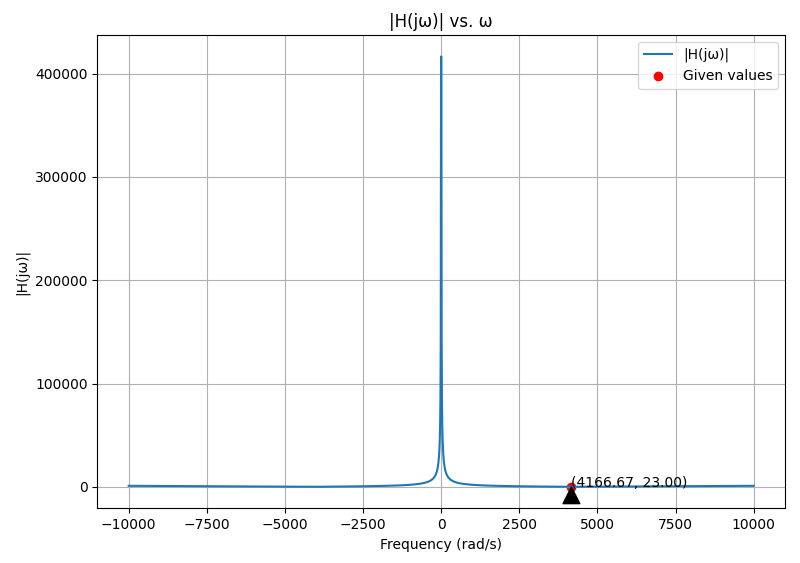
\includegraphics[width=\columnwidth]{figs/analog.png}
  \label{fig:bode_Plot}
\end{figure}

\end{document}

